\documentclass[a4paper, notitlepage]{report}

\usepackage{a4wide}
% To decrease the margins and allow more text on a page.

\usepackage{graphicx}
% To deal with including pictures.

\usepackage{enumerate}
% To provide a little bit more functionality than with LaTeX's default
% enumerate environment.

\usepackage{array}
% To provide a little bit more functionality than with LaTeX's default
% array environment.

\usepackage{multicol}
% For if we want to put something in a multi column environment.

\usepackage[dutch]{babel}
% Use this if you want to write the document in US English. It takes care of
% (usually) proper hyphenation.
% If you want to write your answers in Dutch, please replace 'american'
% by 'dutch'.
% Note that after a change it may be that the first compilation of LaTeX
% fails. That is normal and caused by the fact that in auxiliary files
% from previous runs, there may still be a \selectlanguage{american}
% around, which is invalid if 'american' is not incorporated with babel.

\usepackage{amssymb}
% This package loads mathematical things like the fonts for the blackboard
% bold for the set of natural numbers.

\usepackage{amsmath}
% And some student asked me to include amsmath as well...

\usepackage{verbatimbox}
% For putting verbatim stuff into boxes.

\usepackage{tikz}
\usetikzlibrary{arrows}
\usetikzlibrary{positioning}
% The tikz package can be used to draw all kinds of diagrams.
% For instance parse trees and finite automata.

\usepackage[all]{xy}
% Instead of tikz you can also use xy to draw diagrams.


\usepackage{xspace}
% xspace can be used to let LaTeX decide whether a command should be followed
% by a space or not, depending on what follows.

% Normally subsections are numbered as section.subsection, but because
% we don't have a section, we remove the first part and only show the
% subsection number itself.

\renewcommand{\thesubsection}{\arabic{subsection}}

% Replace the placeholders by your real names, student numbers and
% tutorial groups.
\author{
	Matthijs Muis \\
	s1066918
}

\title{
	Statistiek Inleveropgave \\
	Week 13 en 14
}


\begin{document}

\maketitle
\begin{abstract}
  Ter afronding van de huiswerkopgaven van het vak Statistiek zijn de laatste twee weken gewijd aan een wat groter project. Het doel is om een echte dataset te analyseren en hiervoor een lineair regressiemodel te formuleren. Modelselectie speel dus een centrale rol: welke deelverzamelingen van variabelen hebben samen een hoge verklarende waarde, welke transformaties, interactietermen zijn zinvol.
  
  De punten die genoemd worden in de opdracht zullen een subset zijn van het verslag. Daarnaast wil ik experimenteren met een systematische aanpak voor variable selection. Daarom is er een extra sectie opgenomen met de theoretische achtergrond van de \emph{step-up} en \emph{step-down} methoden, twee zeer vergelijkbare en intu\"itief aansprekende methoden voor het systematisch selecteren van variabelen
\end{abstract}
\clearpage
\tableofcontents
\clearpage

\chapter{Inleiding}  
\section{Dataset}
  Zij eerst opgemerkt dat we als basisdataset nemen de dataset uit $n = 52$ waarnemingen, met voor $i = 1, \dots ,n$ steeds waarneming $(x_i,Y_i)$ waar $x_i \in \mathbb{R}^q$ voor $q = 4 + 2$, $Y_i \in \mathbb{R}$ met:
  \begin{align*}
  x_1 &= 1_{\text{[sector = "Finance"]}} &
  x_5 &= \text{assets} \\
  x_2 &= 1_{\text{[sector = "Energy"]}} &
  x_6 &= \text{marketval} \\
  x_3 &= 1_{\text{[sector = "Manufacturing"]}} &
  y &= \text{sales} \\
  x_4 &= 1_{\text{[sector = "Retail"]}}
  \end{align*}
  
  We zetten de categorische data dus alvast om in binaire data, want dat moet uiteindelijk toch. Maar wanneer het ons uitkomt, roepen we in \verb!R! gewoon de categorische variabele aan. Sterker nog, hier is \verb!R! op gemaakt: \verb!marketval:sector! aanroepen in de command \verb!lm! zal bijvoorbeeld precies 4 interactievariabelen maken als producten $x_1x_6, \ x_2x_6, \ x_3x_6, \ x_4x_6$.
  
  De continue variabelen in de dataset zijn \verb!sales!, \verb!assets! en \verb!marketval!. Dit zijn de \emph{omzet}, het \emph{kapitaal} (in aandelen) en de \emph{marktwaarde} van het bedrijf. Deze economische variabelen hebben de volgende betekenis:
  
\begin{enumerate}
  \item De \emph{(jaar)omzet} van een bedrijf is de nettowinst die het bedrijf in een jaar heeft gemaakt.
  \item Het \emph{kapitaal} van een bedrijf is het totale geldbedrag dat de aandelenverkoop van het bedrijf heeft opgeleverd. Een bedrijf kan aandelen (assets) verkopen op de aandelenbeurs. Een koper van zo'n aandeel heet een aandeelhouder en het bezit van een aandeel betekent dat de aandeelhouder mag delen in de winst van het bedrijf middels een winstuitkering die \emph{dividend} heet. Voor het bedrijf is de aandeelhouder een investeerder en kan het kapitaal besteed worden aan hulpbronnen of uitbreidingen.
  \item De \emph{marktwaarde} van een bedrijf is de theoretische verkoopprijs van het bedrijf, dus een bod welke de markt vindt dat de eigenaar van het bedrijf redelijkerwijs zou kunnen accepteren voor de verkoop van het bedrijf, niet te hoog en niet te laag. Uiteraard is de marktwaarde niet een waargenomen variabele, maar moet deze geschat worden. Dit doen analisten op basis van allerlei data. Wij gaan ervan uit dat deze marktwaarde de `echte' marktwaarde is, voor ons is het dus wel een waarneming.
\end{enumerate}
  
  Tenslotte nog iets over de categorische variabele \verb!sector!: in de Fortune-500 dataset zit categorische variabele die de sector van het bedrijf aangeeft. Er zijn 4 sectoren of, in \verb!R!-jargon, \emph{levels}: \emph{Energy, Finance, Manufacturing} en \emph{Retail}. 
  
  Nu geven we eerst wat marginale verdelingen van deze variabelen met behulp van histogrammen. Deze plots zullen nog weinig informatie geven over het verband tussen de variabelen, maar het is handig om ze alvast bij de hand te hebben. Het maken van dit soort plots kan eenvoudig met de onderstaande commands in de command-line van \verb!R!.

\begin{verbatim}
> barplot(summary(sector))
> hist(marketval)
> hist(sales)
> hist(assets)
\end{verbatim}


\begin{figure}
\begin{center}
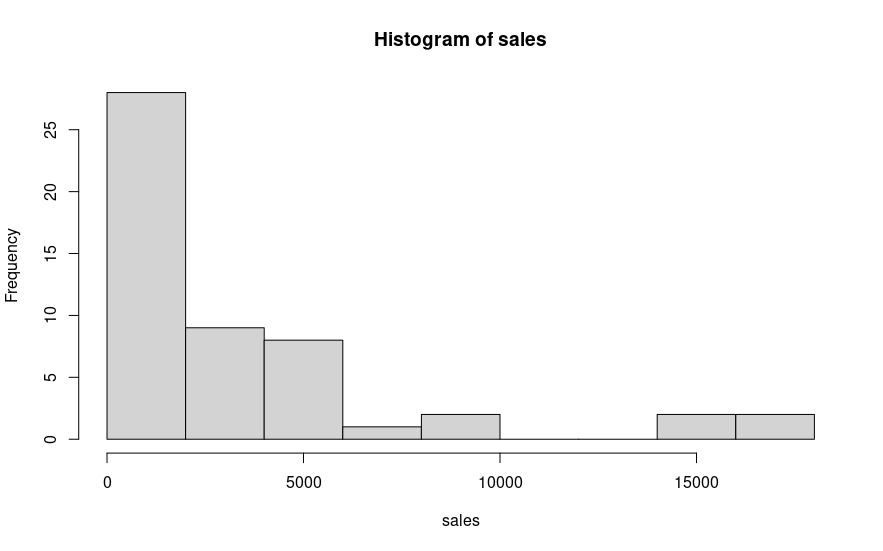
\includegraphics[width=.45\textwidth]{histSales.PNG}
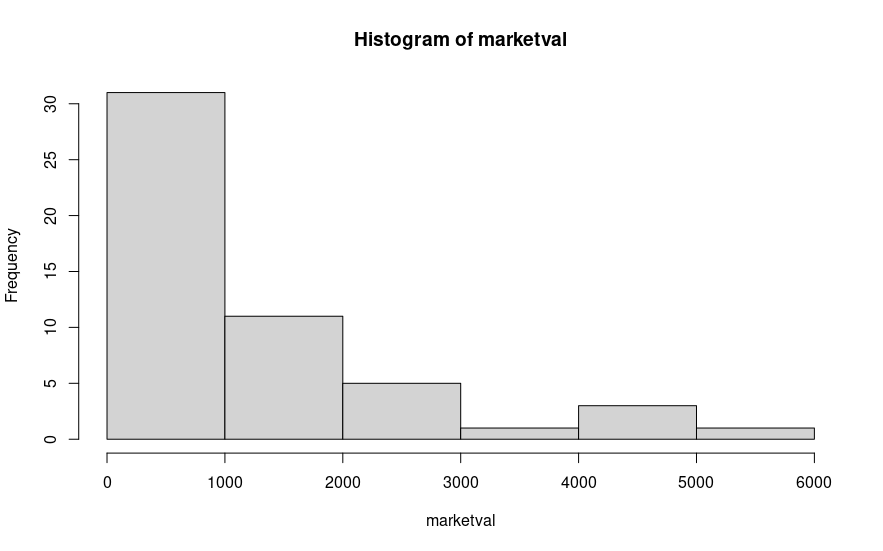
\includegraphics[width=.45\textwidth]{histMarketval.PNG}
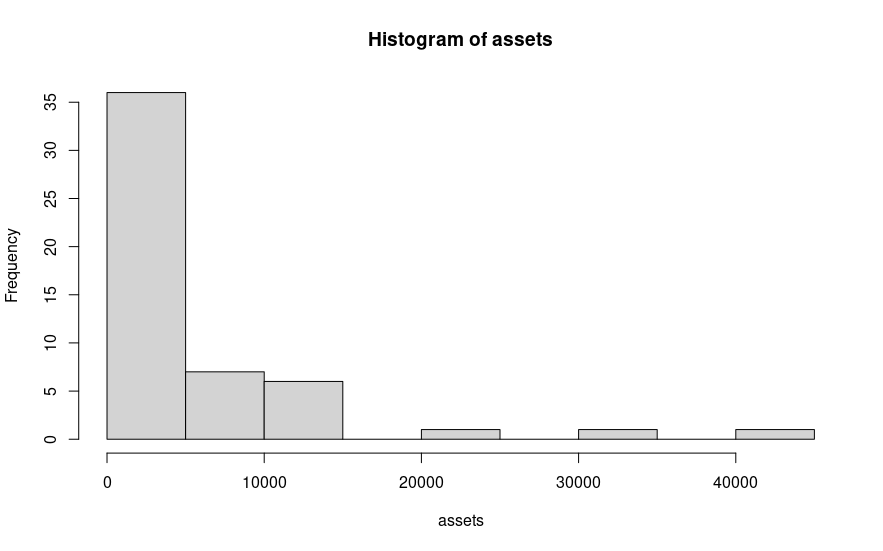
\includegraphics[width=.45\textwidth]{histAssets.PNG}
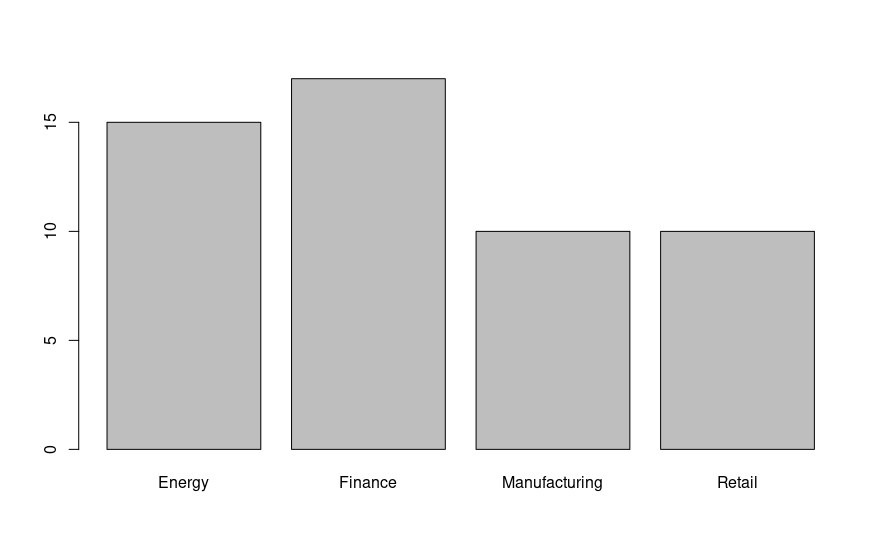
\includegraphics[width=.45\textwidth]{barSector.PNG}
\end{center}
\caption{De marginale verdelingen van de vier gegeven covariaten.}
\end{figure}

  De bovenstaande plots geven als eerste indruk dat de financi\"ele variabelen erg scheef verdeeld zijn. Dit motiveert mogelijk een logaritmische transformatie van de financi\"ele data, waarover we hieronder nog uitgebreid zullen komen te spreken. De logtransformatie wordt echter niet evident gemaakt door de bovenstaande plots Het is bijvoorbeeld goed mogelijk dat de correlatie tussen de continue variabelen ervoor zorgt dat de residuen van het lineaire model t\' och normaal verdeeld blijken te zijn.
  
  Over de precieze modelaannamen hebben we nog niet gesproken, zie hiervoor 1.2. Het moge echter duidelijk zijn dat dit een lineair model wordt met als verklaarde variabele \verb!sales! en als covariaten variabelen die alleen afhangen van \verb!assets!,\verb!marketval! en \verb!sector!. We verwachten in elk geval dat een groter kapitaal en een grotere marktwaarde gecorrelleerd zijn met een grotere omzet. Een bedrijf dat meer te besteden heeft zal meer investeringsmogelijkheden hebben en daardoor meer winst kunnen maken en daardoor waardevoller zijn dan een bedrijf dat minder winst maakt. 
  
  We gaan ons ori\"enteren op dit ruwe vermoeden door wat eendimensionale plots van de continue variabelen tegen elkaar, met een regressielijn ertussen. In feite zijn we hier al twee heel eenvoudige lineaire model aan het fitten, namelijk \verb!sales ~ assets! en \verb!log(sales) ~ log(marketval)! (tenzij anders aangegeven \emph{inclusief} intercept). Beide modellen `zien' echter voor zichzelf slechts \' e\' en van de twee (relevante?) financi\"ele covariaten. Daardoor is de regressielijn in beide gevallen waarschijnlijk biased (zie namelijk de theorie over \emph{restricted models}).
  
\begin{figure}[H]
\begin{center}
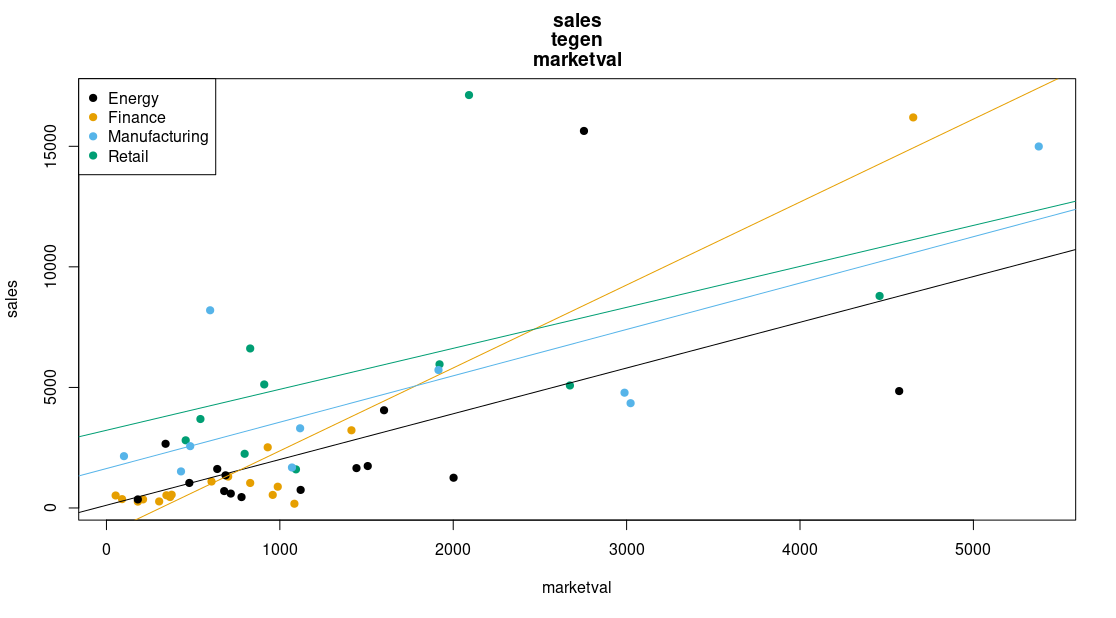
\includegraphics[scale=.25]{salesMarketval.PNG}
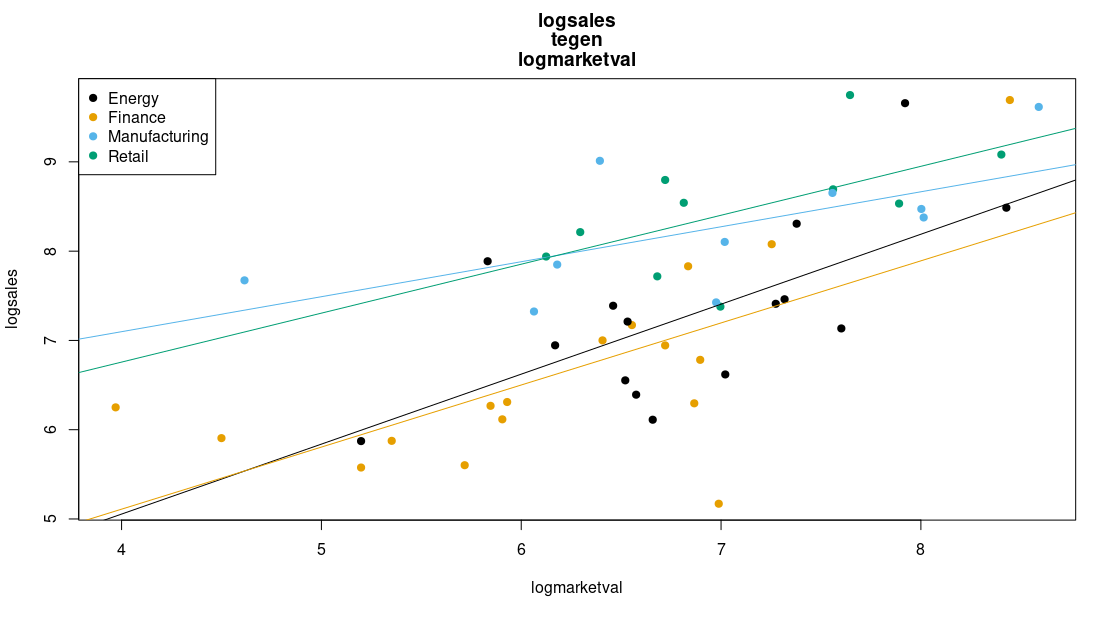
\includegraphics[scale=.25]{logsalesLogmarketval.PNG}
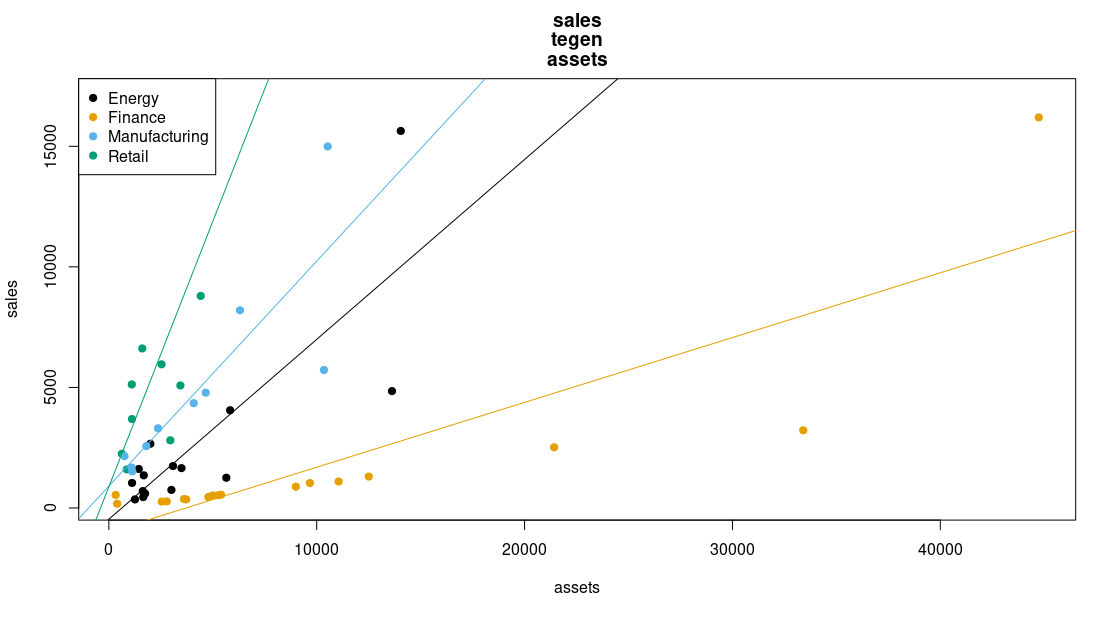
\includegraphics[scale=.25]{salesAssets.PNG}
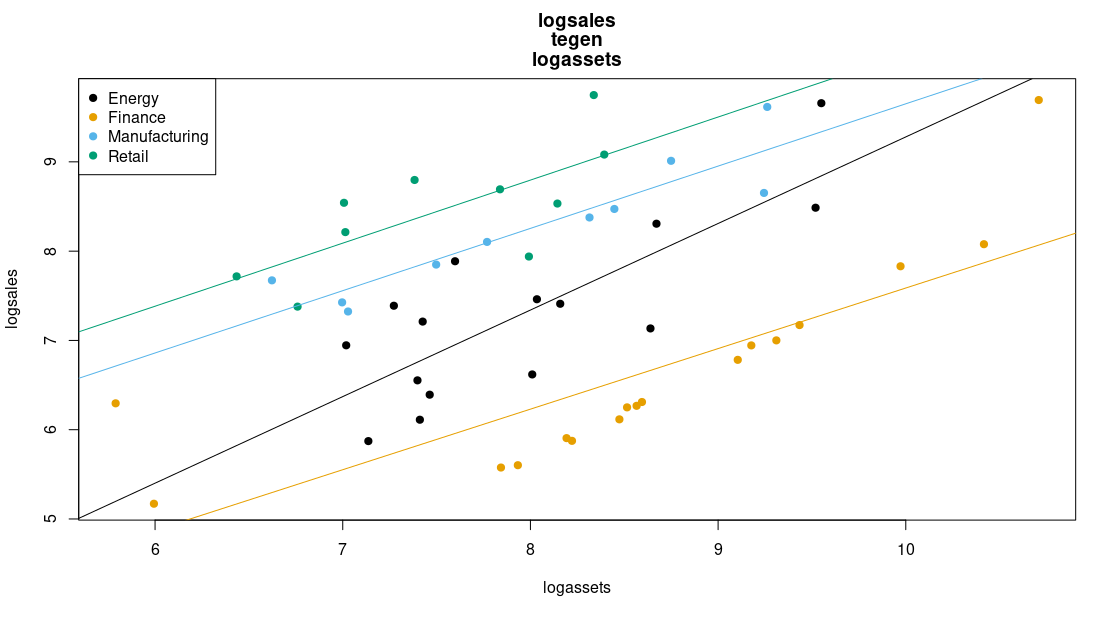
\includegraphics[scale=.25]{logsalesLogassets.PNG}
\end{center}
\caption{Scatterplots van sales tegen marketval, assets respectievelijk. Links zijn de `raw' datapunten genomen, rechts is een $\log$-transformatie toegepast.}
\end{figure}

\begin{figure}
\begin{verbatim}
plot(marketval
     , sales
     , main = "sales tegen marketval"
     , xlab = "marketval"
     , ylab = "sales"
     )
abline(lm(sales ~ marketval))

plot(log(marketval)
     , log(sales)
     , main = "log sales tegen log marketval"
     , xlab = "log marketval"
     , ylab = "log sales"
     )
abline(lm(log(sales) ~ log(marketval)))

plot(assets
     , sales
     , main = "sales tegen assets"
     , xlab = "assets"
     , ylab = "sales"
     )
abline(lm(sales ~ assets))

plot(log(assets)
     , log(sales)
     , main = "log sales tegen log assets"
     , xlab = "log assets"
     , ylab = "log sales"
)
abline(lm(log(sales) ~ log(assets)))
\end{verbatim}
\end{figure}
  
  We zien in alle plots een zwakke trend, maar vooral rechts is deze beter zichtbaar. Links zien we wederom scheefheid in de data, welke duidelijk leidt tot ongewenste \emph{heteroskedasticiteit} in beide modellen. Waarom geen plots van $\log$s tegen niet-$\log$s? Dat is weinig zinvol, blijkt uit 2.1. 

\section{Model}  
  Zij eerst opgemerkt dat we een lineair model zullen schatten met gronddata gegeven in de bovenstaande variabelen, maar dat wanneer we over `covariaten' spreken, we het over de covariaten hebben die op dat moment in dat model gekozen zijn. We doen dus de volgende modelaannamen voor een nog onbekende design-matrix $X \in \mathbb{R}^{n\times p}$ en de datavector $Y \in \mathbb{R}^n$:
  
\begin{align}
  Y = X\beta + \varepsilon \\
  \varepsilon \sim \mathcal{N}(0,\sigma^2I_n)
\end{align}
  
\section{Onderzoeksvragen}
  In dit hoofdstuk gaan we enkele vragen formuleren bij de data die interessant kan zijn bij het analyseren van verbanden in de dataset. Aan de hand van deze vragen kunnen we verdelingsonderzoek verrichten en daarna een aantal kandidaatmodellen formuleren die ons zinvol lijken.
  
  Ik heb me bij het formuleren van de vragen gebaseerd op eigen ingeving alsook op de suggesties uit de opdracht.  
  
  De kernvraag die centraal zullen staan in deze regressie-analyse: wat is de verzameling van zinvolle covariaten die we kunnen bedenken? Deze verzameling begrenst namelijk ons zoekdomein. Zodra we alle covariaten hebben geformuleerd die we in overweging willen nemen, kunnen we testen welke combinaties van covariaten significant zijn
  
\begin{enumerate}
  \item Is een $\log$-transformatie voor elke financi\"ele variabele zinvol?
  
  \item Is er significante variatie conditionele verdelingen van \verb!sales! of anders \verb!logsales! afhankelijk van \verb!sector!? In woorden, heeft de sector van een bedrijf significante invloed op de verwachte omzet van het bedrijf en de onzekerheid (variantie) hiervan?
  
  \item Zie in dit opzicht ook suggestie 6: \emph{is het zinvol om de variantie per categorie te schatten?}. Merk op dat deze variantie $\sigma^2 = \mathbb{E}\Vert \varepsilon \Vert ^2$ natuurlijk pas gedefinieerd is zodra een keuze voor de covariaten (dat is, de vorm van de design-matrix) is gedaan. We zullen dit dus voor ieder geformuleerde model apart moeten onderzoeken. De precieze formulering is dan, of $\varepsilon \sim \mathcal{N}(0,\Sigma^2)$ met $\Sigma^2$ een diagonaalmatrix, maar nu op de diagonaal is $(\Sigma^2)_{ii} = \sigma^2_{\text{sector}}$, welke nog afhangt van de \verb!sector! van datapunt $X_{i-}$. Dit klinkt moeilijk om te implementeren, maar vergeet niet dat \verb!R! gebouwd is voor dit soort vragen (`subsetting' is een magic word!).
\end{enumerate}

  Zoals te zien is, lijken veel van deze vragen pas post-fit te beantwoorden. Of een log-transformatie zinvol is, zien we pas wanneer we kunnen testen of de residuen er `normaler' van worden (denk aan een KS-toets, of visueel, een QQ-plot tegen normale kwantielen). De residuen kennen we pas zodra we een model hebben vastgepind. 
  
  We willen dus dat onze modelkeuze op dat punt op een beetje variatie na bepaald is. Om ons ruimte te geven voor de duidelijk veel interessantere vragen vanaf vraag 2, gaan we eerst de vraag naar het al dan niet transformeren van financi\"ele variabelen tacklen.
  
\chapter{Kandidaatvariabelen en -transformaties}

\section{$\log$-transformatie voor financi\"ele data}
\subsection{Ecomische motivatie voor $\log$-transformatie}
  Er bestaat een heldere motivatie voor het $\log$-transformeren van financi\"ele data. In het geval van financi\"ele data zijn afhankelijkheden veelal ratio en niet additief. Beschouw immers de volgende (zeer eenvoudige) modellen voor de omzet van een bedrijf, afhankelijk van het kapitaal:

\begin{align}
  \text{sales} = \alpha + \beta \cdot \text{assets} \\
  \text{log(sales)} = \alpha + \beta \cdot \text{log(assets)}
\end{align}
  (N.B. deze modellen corresponderen met de twee onderste trendlijnen in figuur 1.2)
  
  Het is intu\"itief aansprekend dat wanneer het kapitaal van een bedrijf met 5\% stijgt, de marktwaarde met een evenredig (niet per se gelijk) percentage zal toenemen. Dit correspondeert met een lineaire verschuiving van $\log(\text{sales})$ (n.l. met $\log(1.05)$), en een daaruit volgende lineaire verschuiving van $\log(\text{sales})$ (n.l. met $\beta \log(1.05)$). Een uitspraak als `wanneer een retailbedrijf in kapitaal verdubbelt, zal de omzet met 50\% toenemen' correspondeert met een $\beta = \log(2)/\log(1.5)$.
  
  Wat het ongetransformeerde lineaire model postuleert, is veel minder aannemelijk. Dit verband houdt namelijk in dat per extra 1\$ in omzet de marktwaarde met $\beta$\$ zal stijgen. Maar niet voor elk kapitaalniveau zal elke extra dollar direct omgezet worden in $\beta$ extra dollar winst, om het maar even grof te formuleren. Deze toename per extra dollar noemen economen de `marginale omzet' (wij noemen het de afgeleide), en een van de centrale aannamen in de economie is juist de wet van `diminishing returns', dus dat deze marginale omzet afneemt. 
  
  Een motivatie voor deze wet is eenvoudig: bij toename van het kapitaal naar een steeds groter bedrag, zullen toch andere variabelen - zoals begrensde afzetmogelijkheden - beperkingen opleggen aan de winst. Neem bijvoorbeeld MacDonalds: dit bedrijf kan met meer kapitaal weliswaar meer restaurants openen, meer reclamezuilen huren en in nog goedkopere productiemethoden voor burgers investeren en met nog meer kwantumkorting aardappel(meel) inkopen om er frietjes van te maken, uiteindelijk is er een grens aan het aantal bezoeken per persoon per dag en dus aan de verkoop van producten. Het kan dus niet anders of de `(kapitaal $\mapsto$ winst)-functie' zal ergens beginnen te krommen naar een asymptoot.
  
  
  Het is moeilijk om deze kromming waar te nemen in de gegeven data, dus voor deze subsection zal het helaas blijven bij wat economisch gefilosofeer. De volgende motivatie voor de $\log$-transformatie is statistisch van aard en zullen we op rigoreuze wijze hard maken.
  
  Tenslotte moeten we ook de mogelijkheid overwegen om alleen de verklarende of alleen de verklaarde variabele te transformeren. Dit heeft echter geen zinvolle economische interpretatie en is daardoor moeilijk te rechtvaardigen. Bovendien worden twee verschillende eenheden met elkaar in verband gebracht: namelijk geld en ratio's van geld. Dat is ook niet erg logisch. Het komt in praktijk dan ook nooit voor.
 
\subsection{Statistische motivatie voor de $\log$-transformatie} 
  Een andere motivatie van het nemen van $\log$-transformaties heeft meer te maken met de verdeling van het logaritme van financi\"ele data. Financi\"ele data blijkt in praktijk heel scheef verdeeld te zijn. Wederom is dat logisch, want in een groot bedrijf met veel kapitaal passen veel kleine bedrijfjes met weinig kapitaal. De verhouding bedrijven met `groot kapitaal' tot bedrijven `klein kapitaal' is daardoor scheef. 
  
  Deze observatie deden we al toen we keken naar de marginale verdelingen van de financi\"ele variabelen in onze dataset (zie 1.1). We zagen de scheefheid terugkomen in de uitbijters in het scatterplot van de ongetransformeerde data.
  
  Deze uitbijters zijn desastreus voor de gepostuleerde modelaanname van \emph{homoskedasticiteit}, d.w.z. de variantie van de residuen is constant en niet gecorrelleerd met de grootte van de covariaten. Immers, als het logaritme van elke financi\"ele variabele, zeg $Z$ een vaste verdeling volgt, zoals een normale verdeling, dan volgen de financi\"ele variabelen de verdeling van $\exp(Z)$. De $\exp$-functie kromt sterk naar boven voor grotere waarden van $Z$, dus bij kleine variatie van $Z$ rond een bepaald punt $x$ is variatie van $\exp(Z)$ klein voor kleine waarden van $x$ en juist heel groot voor grote waarden van $x$. dus als $\text{log(sales)} = \alpha + \beta \cdot \text{log(assets)}$ voldoet aan homoskedasticiteit, dan $\text{sales} = \alpha + \beta \cdot \text{assets}$ z\' eker niet!
  
  We kunnen echter veel rigoureuzere uitspraken doen over deze financi\"ele variabelen met statistische toetsen. Ik wil zelfs beweren dat de marginale verdelingen van de $\log$s van de financi\"ele data inderdaad normaal zijn. Nu gaan we een Kolgomorov-Smirnov-toets uitvoeren om dit te toetsen voor de marginale verdelingen van \verb!assets!, \verb!marketval! en \verb!sales!.
  
\subsection{Kolgomorov-Smirnov-toets op normaliteit van logassets, logmarketval en logsales}  
  
  Het idee achter de KS-toets is bekend uit \emph{Inleiding in de Statistiek}. Voor $H_0: F = F_0, \ H_1: F \neq F_0$: zij $T$ de grootste absolute afwijking tussen de empirische verdelingsfunctie van de data en de nulverdeling $F_0$, dan volgt $T$ een bekende verdeling en verwerpen we voor $T$ groot genoeg.
  
  Het probleem met de KS-toets, welke ook in dat boek wordt behandeld, is dat men $F_0$ eigenlijk graag wil kiezen op basis van geschatte parameters n\' adat men de data heeft waargenomen. Wij willen nu bijvoorbeeld controleren of \verb!assets! een normale verdeling bezit, en als $F_0$ willen we graag de verdeling kiezen die als gemiddelde en variantie het waargenomen steekproefgemiddelde en de waargenome variantie van \verb!assets! bezit. Dit mag niet, omdat $F_0$ een vaste verdeling moet zijn die niet mag afhangen van de data dus ook niet van de schatters $\bar{X_n}$ en $S^2_X$.
  
  Een uitbreiding van de KS-statistiek $T^*$ (zie wederom \emph{Inleiding in de Statistiek}) is gegeven voor het tupel van hypothesen $H_0: F = F_{\theta}, \ H_1: F \neq F_{\theta}$. $T^*$ is nu de grootste absolute deviatie tussen de empirische verdelingsfunctie en de verdelingsfunctie die geparametriseerd is door de maximum-likelihoodschatters van de parameters. In praktijk zijn deze voor een normale verdeling $\overline{X_n} en S_X$ en geeft dit de volgende toetsingsgrootheid:

  \begin{equation}
    T^* = \sup_{x\in \mathbb{R}} | \mathbb{F}_n(x) - \Phi(\frac{x-\overline{X_n}}{S_X}|
  \end{equation}  	
	
   We zijn nu ge\"interesseerd in de verdeling van $T^*$ onder de nulhypothese, zodat we bij zeer incompatibele waarden van $T^*$ de nulhypothese kunnen verwerpen en een $p$-waarde kunnen geven. Merk echter op dat de verdeling van $T^*$ in zijn geheel niet triviaal is. We zouden deze kunnen simuleren, maar ook dan is de vraag met welk element (welke normale verdeling dus) van $\mathcal{F}$ we dit zouden moeten doen. Immers hangt de verdeling van $T^*$ misschien wel af van de ware parameter van de normale verdeling? 
   
   Op p.146 van \emph{Inleiding in de Statistiek} staat gelukkig dat de verdeling van $T^*$ hetzelfde is onder ieder element van de nulhypothese. We nemen dus een standaardnormale verdeling en bepalen met behulp van simulatie de nulverdeling van $T^*$:

  Vervolgens bepalen we de KS-test statistiek met de ingebouwde functie in \verb!R!. Dit doen we voor \verb!assets!, \verb!marketval! en \verb!sales!, en dus ook voor \verb!logassets = log(assets)!, \verb!logmarketval = log(marketval)! en \verb!logsales = log(sales)!: onze implementatie gaat andersom te werk en verschuift en schaalt eerst de waargenomen data met het steekproefgemiddelde en de steekproefstandaarddeviatie, en berekent daarna de KS-statistiek met de standaardnormale verdeling. Dit levert hetzelfde getal op maar ziet er in \verb!R! wat eleganter uit.
	
  \begin{figure}
  \begin{verbatim}
# Simuleer een steekproef van N realisaties van T* onder de nulhypothese
# bij een steekproefgrootte van n uit een normale verdeling
NullExtendedKS <- function(N, n){
  D = numeric(N)
  for (i in 1:N){
    X <- rnorm(n)
    D[i] <- ks.test((X - mean(X))/sd(X), pnorm)$statistic
  }
  return(D)
}


N <- 1000000
n <- 52

logsales = log(sales)
logassets = log(assets)
logmarketval = log(marketval)


Tlogsales <- ks.test((logsales - mean(logsales))/sd(logsales), pnorm)$statistic
Tlogassets <- ks.test((logassets - mean(logassets))/sd(logassets), pnorm)$statistic
Tlogmarketval <- ks.test((logmarketval - mean(logmarketval))/sd(logmarketval), pnorm)$statistic

Tsales <- ks.test((sales - mean(sales))/sd(sales), pnorm)$statistic
Tassets <- ks.test((assets - mean(assets))/sd(assets), pnorm)$statistic
Tmarketval <- ks.test((marketval - mean(marketval))/sd(marketval), pnorm)$statistic

D = NullExtendedKS(N,n)


hist(D, , probability = TRUE, breaks = 50)

lines(c(Tlogsales,Tlogsales), c(0,N), lwd = 2, col = "darkorange")
lines(c(Tlogassets,Tlogassets), c(0,N), lwd = 2, col = "chartreuse")
lines(c(Tlogmarketval,Tlogmarketval), lwd = 2, c(0,N), col = "blue")

lines(c(Tsales,Tsales), c(0,N), lwd = 2, col = "purple")
lines(c(Tassets,Tassets), c(0,N), lwd = 2, col = "magenta")
lines(c(Tmarketval,Tmarketval), c(0,N), lwd = 2, col = "darkred")
  \end{verbatim}
  \captio{Het R-script. Als je het runt, geeft R voor elke KS-test die je uitvoert met geschatte parameter een warning voor `ties'. Maar wij doen niet de test van R, maar willen alleen de statistiek weten. Deze warnings zijn dus niet van toepassing!
  \end{figure}
  
  \begin{figure}
  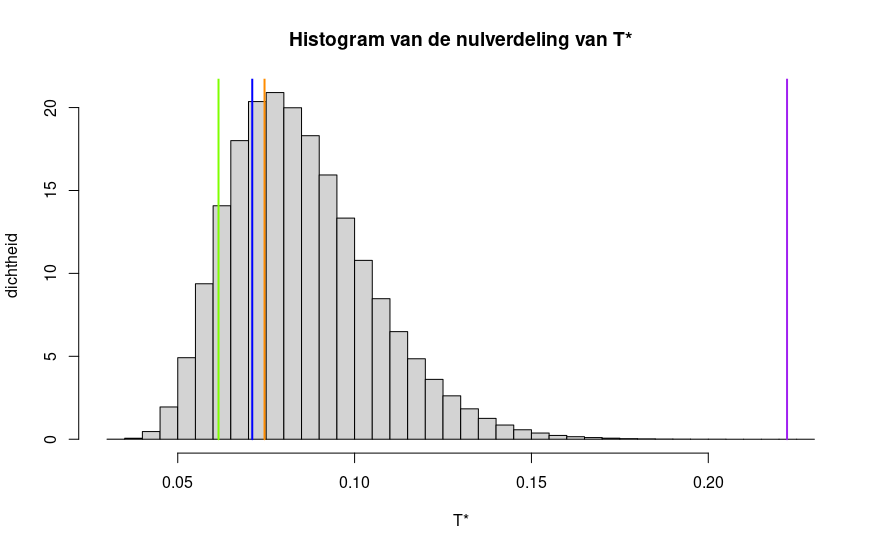
\includegraphics[scale=.5]{KSTestLog.PNG}
  \caption{De nulverdeling van $T^*$. De lijnen geven de werkelijke waarden van $T^*$ aan zoals berekend voor de financi\"ele en logfinanci\"ele variabelen. De kleuren corresponderen met:
    \begin{enumerate}
      \item groen: 
      \item blauw:
      \item oranje:
      \item paars, rood, magenta: overlappen elkaar, dit zijn de ongetransformeerde variabelen.
    \end{enumerate}
  \end{figure}
  
  De $p$-waarden vinden we als:
  \begin{figure}
  \begin{verbatim}
pvalue <- function()
{
  return (sum(D>t)/N) #verwerp voor grote waarden van D
}

pvalue(Tlogsales)
pvalue(Tlogassets)
pvalue(Tlogmarketval)

pvalue(Tsales)
pvalue(Tassets)
pvalue(Tmarketval)

> pvalue(Tlogsales)
[1] 0.663722
> pvalue(Tlogassets)
[1] 0.897291
> pvalue(Tlogmarketval)
[1] 0.734819
> 
> pvalue(Tsales)
[1] 1e-06
> pvalue(Tassets)
[1] 0
> pvalue(Tmarketval)
[1] 0
  \end{verbatim}
  \end{figure}
  
  We kunnen dus niet verwerpen dat de logaritmes normaal verdeeld zijn, terwijl we heel zeker kunnen verwerpen dat de ongetransformeerde variabelen normaal verdeeld zijn.
	
  Ik wilde nog een QQ-plot maken maar dat is nu wel overbodig. We gaan door! Gooi de oorspronkelijke data uit het raam. We werken voortaan met de logaritmes.
  
  \begin{figure}
  \begin{verbatim}
> remove(sales, assets, marketval)
  \end{verbatim}
  \end{figure}
	
  N.B. Later zullen we interactievariabelen van de sectoren met de financi\"ele covariaten invoeren. Als we het voorgaande echt netjes hadden willen doen, hadden we dus eigenlijk moeten controleren of de conditionele verdeling van elk financi\"ele covariaat geconditioneerd naar \verb!sector! normaal is na een $\log$-transformatie. Dan zouden we echter 12 toetsen moeten uitvoeren, en daar is met het oog op de andere dingen die ik nog wil doen in dit onderzoek geen ruimte voor.
  
\section{Kandidaatvariabelen}
  We hebben 3 gegeven verklarende variabelen, waarvan een met 4 levels en de overige continu. We hebben dus 6 variabelen die we in producten, kwadraten, `gewone' termen etc. kunnen verwerken. Toch is uiteindelijk slechts een beperkte verzameling covariaten betekenisvol en daarvan is slechts een bepaalde combinatie significant verklarend. 
 
  We moeten ons zoekveld van tevoren dus beperken tot covariaten en combinaties daarvan die zinnig lijken. In deze sectie zullen we de collectie van deze termen verzinnen en deze vervolgens samenstellen tot een aantal kandidaatmodellen. In latere hoofdstukken worden deze modellen getest en eventueel bijgesteld. We zullen ze hieronder wel alvast schatten
  
\subsection{Geen interactie: het eenvoudigste model}
  Het eenvoudigst mogelijke model dat alle gegeven variabelen uit de dataset gebruikt, heeft als covariaten \verb!logassets!,\log!marketval! en 4 dummy's voor de 4 levels van \verb!sector!. Er is geen interactie tussen de variabelen. Als we dit model schatten in \verb!R!, geeft dit de volgende samenvatting:
  \begin{figure}
  \begin{verbatim}
Call:
lm(formula = logsales ~ logmarketval + logassets + sector)

Residuals:
    Min      1Q  Median      3Q     Max 
-0.8064 -0.3430 -0.1136  0.2910  1.1818 

Coefficients:
                    Estimate Std. Error t value Pr(>|t|)    
(Intercept)          0.67694    0.66809   1.013 0.316244    
logmarketval         0.27718    0.09436   2.937 0.005157 ** 
logassets            0.59310    0.09065   6.543 4.43e-08 ***
sectorFinance       -0.85830    0.21671  -3.961 0.000258 ***
sectorManufacturing  0.90871    0.21757   4.177 0.000130 ***
sectorRetail         1.34954    0.22439   6.014 2.76e-07 ***
---
Signif. codes:  0 ‘***’ 0.001 ‘**’ 0.01 ‘*’ 0.05 ‘.’ 0.1 ‘ ’ 1

Residual standard error: 0.5327 on 46 degrees of freedom
Multiple R-squared:  0.8151,	Adjusted R-squared:  0.795 
F-statistic: 40.56 on 5 and 46 DF,  p-value: 9.248e-16
  \end{verbatim}
  \end{figure}
  
  We zien dat alle variabelen een significantieniveau van minstens 0.001 hebben op \verb!logmarketval! en de \verb!Intercept! na, maar alleen \verb!Intercept! heeft een onacceptabel laag significantieniveau. 
  
  Bij welke tests horen deze $p$-waarden eigenlijk? \verb!R! wil voor elke co\"effici\"ent $\beta_i$ in de parameter $\beta$ toetsen of deze ongelijk is aan 0 ($H_0:\beta_i = 0, \ H_1:\beta \neq 0$), dus of de corresponderende covariaat de variatie in $Y$ significant verklaart. De toets die hiervoor wordt uitgevoerd, is de $t$-toets met statistiek $T = \frac{ \hat{beta}_i - 0}{\sqrt{S^2(X^TX)^{-1}_{ii}}}$, welke onder $H_0$ een $t_{n-p}$-verdeling volgt, voor $n$ de steekproefgrootte en $p$ het aantal covariaten (de `lengte' van $\beta$).
  
\subsection{Effecten van financi\"ele factoren per sector}
  Een redelijke veronderstelling is dat de effecten van de marktwaarde en het kapitaal op de omzet ongelijk zijn tussen de verschillende sectoren. Dit heeft te maken met de werking van bedrijven in verschillende sectoren: 

  \begin{enumerate}
    \item Retailbedrijven hebben over het algemeen een kleinere asset-base ten opzichte van hun omzet, omdat ze veel inkopen en direct weer verkopen. Denk aan een supermarkt: het gros van het kapitaal zit in producten die (soms binnen een dag) verkocht (moeten) worden. Kengetallen als inventory turnover zijn in deze sector heuse prestatiematen.
    
    \item Aan de andere kant van het spectrum zien we financi\"ele bedrijven als banken, verzekeraars, die geld verdienen uit investeringen en rente daarop. Om risico's te dekken hebben zij juist expres een grote `buffer'. Centrale banken hanteren zelfs strikte kengetallen die het eigen vermogen van banken, pensioenfondsen ten opzichte van hun uitstaande investeringen groot moet houden (`vereiste eigen vermogen')
\end{enumerate} 
  
  We vangen dit verschil in effecten door per sector een eigen co\"effici\"ent voor \verb!logassets!. Dit introduceert dus 4 interactietermen in het model, in \verb!R! genoteerd met \verb!logassets:sector!. In dat geval verdwijnt de enkelvoudige regressor \verb!logassets! uit het model, anders heeft de designmatrix geen volledige rang meer.
  
  Het volgende wat we ons kunnen afvragen is of het effect van marktwaarde op de omzet verschilt per sector. Dit is moeilijk te rechtvaardigen: in de marktwaarde zit het verband tussen omzet en sector al `verwerkt', in zekere zin, want het bedrijf is waard wat de koper ervoor wil geven. Als een koper bereid is meer te betalen voor het ene bedrijf dan het andere, dan zal de koper al rekening hebben gehouden met de omzet en de sector waarin het bedrijf zit en wat hij redelijkerwijs als omzet kan verwachten.
  
  We kunnen echter zeker controleren of deze hypothese bevestigt wordt door een lineair model. De ongelijk-aan-0-t-test op de co\"effici\"enten van \verb!logmarketval:sector!  moeten dan niet-significant zijn.
  
\subsection{Drievoudige interactie tussen logmarketval, logassets en sector}
  Een ander idee is dat het effect van het kapitaal of van de marktwaarde op de omzet ook sterker of juist zwakker wordt naarmate de andere financi\"ele variabele groter wordt. Als we dan ook nog het effect per sector willen bekijken, krijgen we een drievoudige interactievariabele in het model, wat correspondeert met 4 covariaten, namelijk gevormd door het product van 4 dummy's en \verb!logmarketval! en \verb!logassets!. Dit effect zouden we kunnen opnemen in het model. We kunnen echter al 5 zinvolle modellen maken met de voorgaande variabelen, en deze term is enigszins vergezocht. Met oog op de lengte van dit project is daarom besloten deze weg niet verder in te slaan.

\subsection{Kwadratische termen en andere machten}
  Deze ga ik niet overwegen: er is in de log-getransformeerde data geen evidente kromming waarneembaar. Bovendien is het nemen van een kwadraat van een logaritme hetelfde als: $(\log(x))^2 = \log(x)\log(x) = \log(x^{\log(x)})$. Hier kunnen we geen interpretatie aan geven. Het is misschien een leuke manier om de $SS_{res}$ omlaag te brengen maar verder niets. 
  
   
\chapter*{Kandidaatmodellen}
  Dit hoofdstuk bevat een overzicht van de modellen die we gaan fitten en hun summary's. Ook zijn er wat plots gemaakt van de residuals. In het volgende hoofdstuk wil ik ingaan op wat extra theorie om een besluit te vormen over het `beste' model, en daarna pas maken we een afweging.
  
\subsection{Model 1}
\begin{verbatim}
  logsales ~ logmarketval + logassets + sector
\end{verbatim}
  Model 1 is het eenvoudigst mogelijke model dat toch alle covariaten gebruikt. Dit model gaat uit van een direct lineair verband tussen \verb!logsales! en \verb!logmarketval!, \verb!logassets!, en heeft dummy's voor elke sector. Er zijn geen interactietermen. De samenvatting van dit model is al te vinden in het voorgaande hoofdstuk en zal hier kortheidshalve niet worden herhaald. Wel geven we een histogram en een QQ-plot van de residuen, en vermelden we de p-waarde van, en de aangepaste KS-statistiek $T^*$ voor normaliteit (let op, dit is een zelfgedefinieerde functie):
  
  \begin{figure}
  \begin{center}
    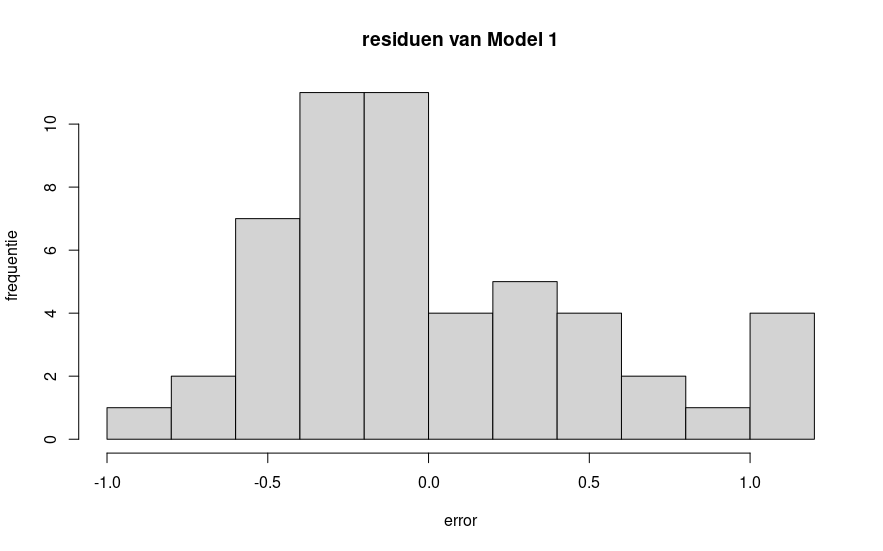
\includegraphics[scale=.45]{histResM1.PNG}
    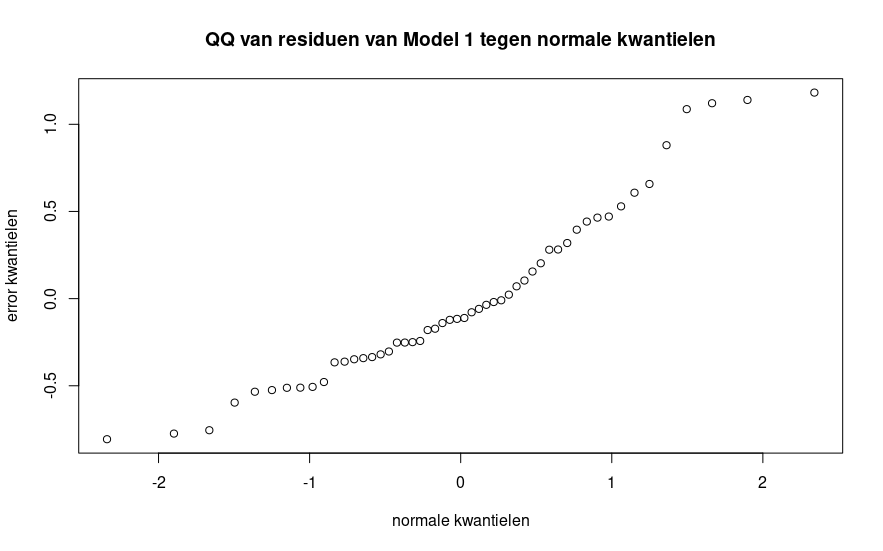
\includegraphics[scale=.45]{qqResM1.PNG}
  \end{center}
  \begin{verbatim}
> pvalue(ks.test((M1$resid - mean(M1$resid))/sd(M1$resid), pnorm)$statistic)
[1] 0.046824
  \end{verbatim}
  \end{figure}
  
\subsection{Model 2}
\begin{verbatim}
  logsales ~ logmarketval + logassets:sector
\end{verbatim}
  Model 2 gaat uit van aparte effecten van \verb!logassets! per sector en een gemeen effect van \verb!logmarketval!. Er is een gemene intercept, de dummy-intercepts uit Model 1 zijn verdwenen.
  
  \begin{figure}
  \begin{center}
    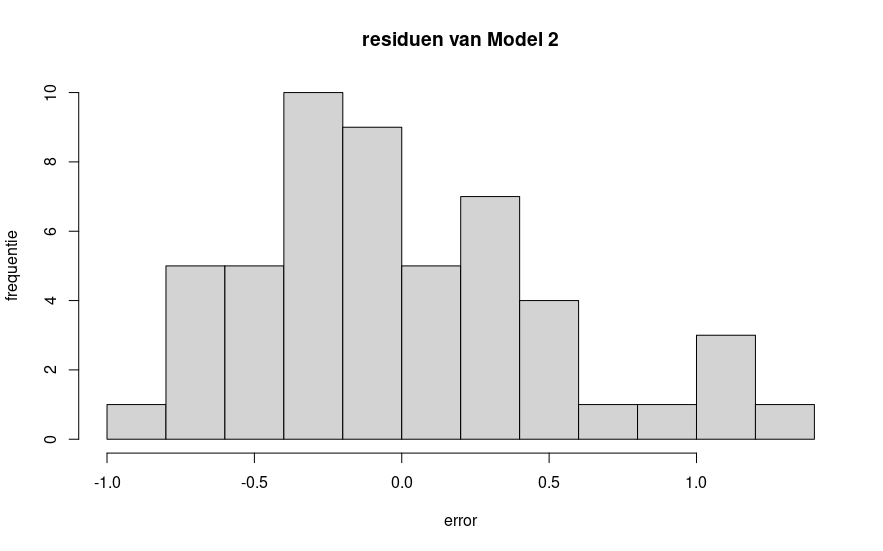
\includegraphics[scale=.45]{histResM2.PNG}
    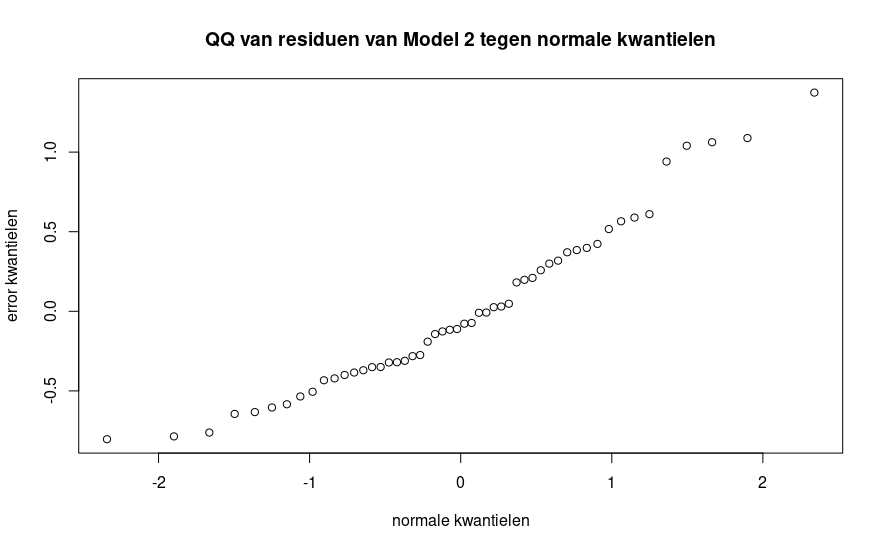
\includegraphics[scale=.45]{qqResM2.PNG}
  \end{center}
  \begin{verbatim}
> pvalue(ks.test((M2$resid - mean(M2$resid))/sd(M2$resid), pnorm)$statistic)
[1] 0.168999
  \end{verbatim}
  \end{figure}
  
\subsection{Model 3}
\begin{verbatim}
  logsales ~ logmarketval:sector + logassets
\end{verbatim}
  Model 3 overweegt juist de aparte effecten van \verb!logmarketval! per sector en houdt het effect van \verb!logassets! gemeen. Er is een gemene intercept.
  
  \begin{figure}
  \begin{center}
    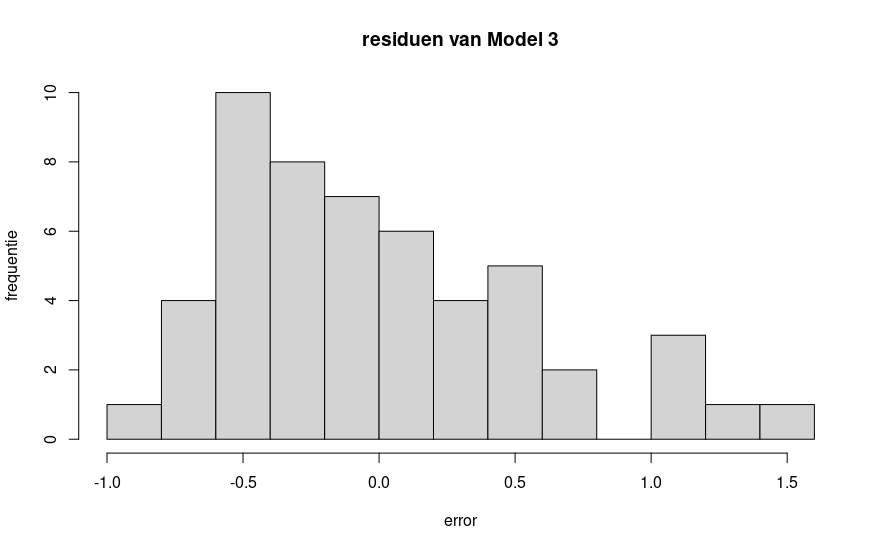
\includegraphics[scale=.45]{histResM3.PNG}
    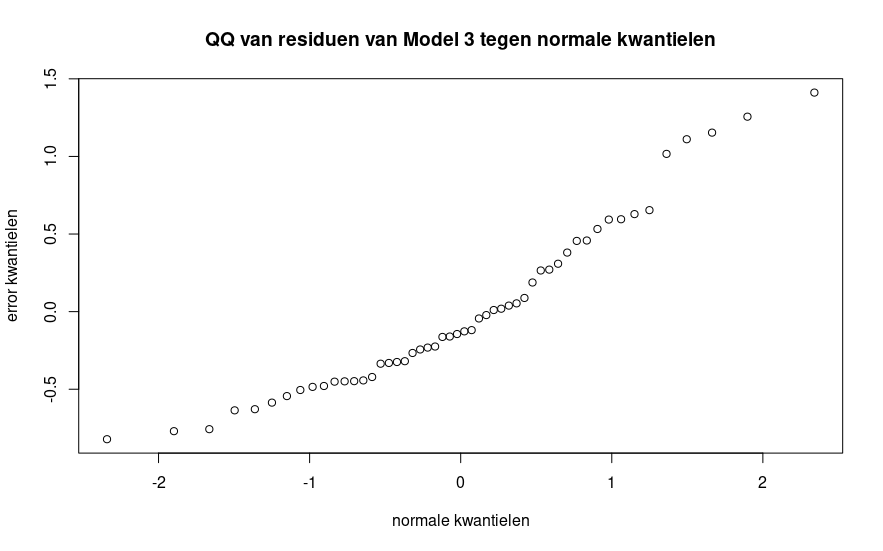
\includegraphics[scale=.45]{qqResM3.PNG}
  \end{center}
  \begin{verbatim}
> pvalue(ks.test((M3$resid - mean(M3$resid))/sd(M3$resid), pnorm)$statistic)
[1] 0.043823
  \end{verbatim}
  \end{figure}
  
\subsection{Model 4}
\begin{verbatim}
  logsales ~ logmarketval:sector + logassets:sector
\end{verbatim}
  Model 4 kan worden gezien als de vereniging van Model 2 met Model 3: er is de interactie \verb!logassets:sector! zoals in 2 en de interactie \verb!logmarketval:sector! zoals in 3
  
  \begin{figure}
  \begin{center}
    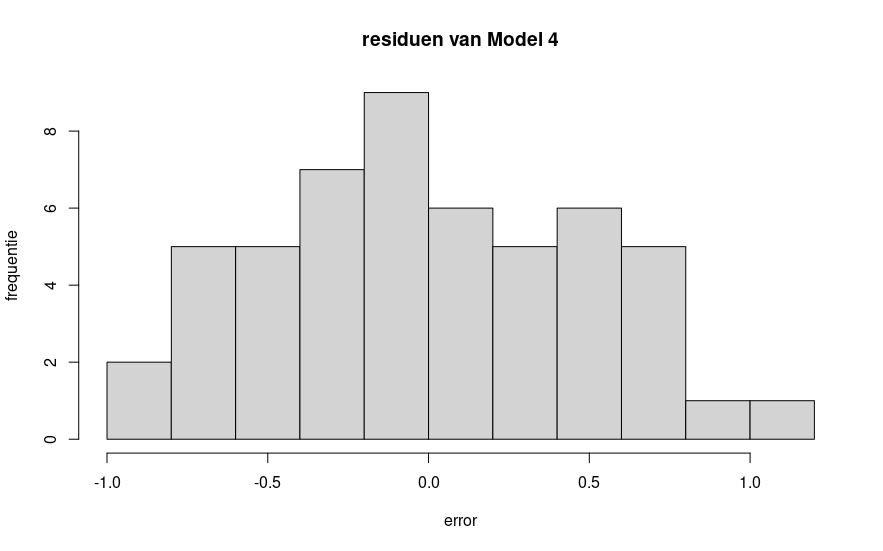
\includegraphics[scale=.45]{histResM4.PNG}
    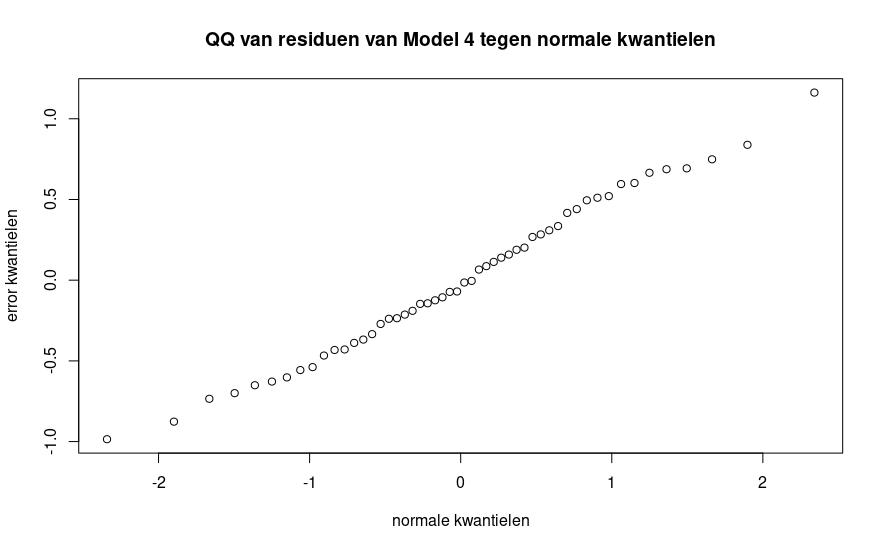
\includegraphics[scale=.45]{qqResM4.PNG}
  \end{center}
  \begin{verbatim}
> pvalue(ks.test((M4$resid - mean(M4$resid))/sd(M4$resid), pnorm)$statistic)
[1] 0.949065
  \end{verbatim}
  \end{figure}
  
\subsection{Model 5}
\begin{verbatim}
  logsales ~ logmarketval + logassets:sector + sector
\end{verbatim}
  Model 5 is geformuleerd na Model 4, en houdt de interactievariabelen en gemene effecten van Model 2 aan. Er is daarnaast een extra intercept per sector opgenomen.
  
  \begin{figure}
  \begin{center}
    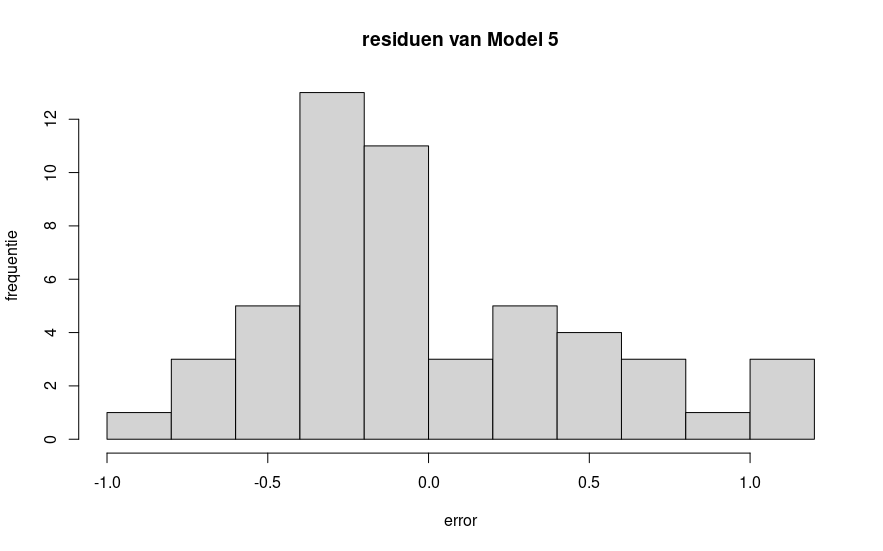
\includegraphics[scale=.45]{histResM5.PNG}
    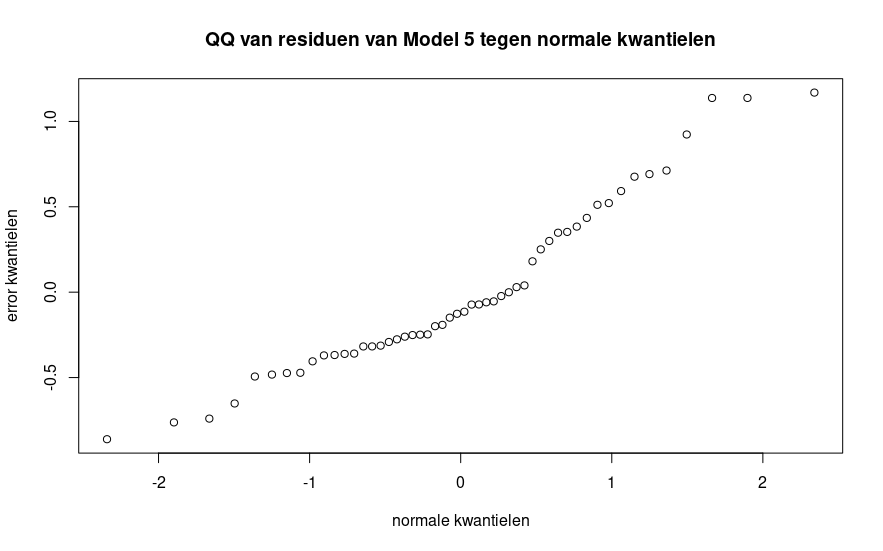
\includegraphics[scale=.45]{qqResM5.PNG}
  \end{center}
  \begin{verbatim}
> pvalue(ks.test((M5$resid - mean(M5$resid))/sd(M5$resid), pnorm)$statistic)
[1] 0.010652
  \end{verbatim}
  \end{figure}
  
\subsection{Eerste indrukken}
  We merken op dat de aanname van homogene normaliteit van de residuen in praktijk niet erg netjes uitpakt: Voor alle modellen behalve Model 5 is de p-waarde van de aangepaste KS-test voor normaliteit van de residuen weliswaar niet altijd klein genoeg om normaliteit te verwerpen, maar wel erg klein (in Model 1 en 3 wordt normaliteit zelfs verworpen).
  
  We zien dat \verb!marketval:sector! in zijn eentje zeer sterk verklarend lijkt (alle co\"effici\"enten worden in de summary van Model 3 als erg significant aangeduid) maar in combinatie met \verb!assets:sector! juist helemaal geen toegevoegde waarde heeft: het kan bijvoorbeeld zijn dat onderliggende correlatie tussen marktwaarde en kapitaal ervoor zorgt dat marktwaarde `de rol van kapitaal overneemt' in Model 3, om vervolgens weer van geen betekenis te zijn n\' a\' ast kapitaal in Model 4.
  
  Model 5 lijkt te groot. Veel co\"effici\"enten verliezen hun significantie ten opzichte van eerdere modellen. De verklaring is dat de variantie van $\hat{\beta}$ toeneemt als we meer vrijheden opnemen in het model, waardoor meer onzekerheid ontstaat over de werkelijke waarde van de parameter. In het hieropvolgende hoofdstuk ga ik daar verder op in.

\chapter*{Theorie: restricted models}
  We hebben gezien dat sommige covariaten op zichzelf erg significant zijn, maar dat wanneer we andere variabelen aan het model toevoegen, deze covariaten juist weer afnemen in significantie. 
  
  Dit maakt kleinere modellen niet per definitie beter, want het kan zijn dat andere covariaten die niet in het model zijn opgenomen werkelijk meer verklarend zijn, en dat we dus een onzuiver (`biased') beeld krijgen van de rol van de covariaten die wel in het model zijn opgenomen: die laatste worden dan te belangrijk geschat. 
  
  Anderzijds neemt de variantie van de schatter van $\beta$ toe naarmate $\beta$ `langer wordt', waardoor het moeilijker wordt om in te schatten welke parameters werkelijk significant zijn: ze kunnen namelijk allemaal als insignificant worden geschat doordat hun variantie zo groot is. Een theoretische verklaring hiervan die iets verder gaat dan de inhoud van hoofdstuk 7 wil ik graag geven in dit hoofdstuk.
  
\section{Theoretisch kader voor het restricted model}
  
\section{De winnaar is...}
  
\chapter*{Variantie per sector}
  In het hoofdstuk waarin de kandidaatmodellen werden voorgesteld, werd steeds een indruk gegeven van de verdeling van de residuen. Normaliteit van deze verdeling werd vaak net niet verworpen door de Lilliefors-test, wat enigszins wrang is als we kijken naar de modelaanname van heteroskedastisch normaalverdeelde errors.
  
  Een mogelijke verklaring is dat de errors niet uit \' e\' en normale verdeling afkomstig zijn, maar uit een mix van normale verdelingen, namelijk per sector is er een `eigen verdeling' voor de errors die voor elke sector mean 0 maar een andere variantie heeft.
  
  Deze verklaring is economisch te interpreteren als: in verschillende sectoren is er verschillende onzekerheid over de mate waarin ons model verklarend is. Sommige sectoren gedragen zich `netjes' ten opzichte van het model: daar zijn marktwaarde en kapitaal sterk verklarend voor de omzet, onze voorspelling wijkt daar meestal niet veel af van de werkelijkheid. Andere sectoren zijn heel `wild': gegeven de marktwaarde en het kapitaal kunnen we eigenlijk niet veel zeggen over de omzet.
  
  Hoe kunnen we toetsen op deze `heteroskedasticiteit tussen sectoren'? Gegeven in de opdracht is de volgende toetsingsgrootheid:
  
  \begin{equation*}
    T = (n-k)\log(\frac{SS_{text{res}}}{n-k}) - \sum_{i=1}^4 (n_i-k_i)\log(\frac{SS_{text{res}}^{(i)}}{n_i-k_i}
  \end{equation*}

  Hierbij is $n$ de steekproefomvang, $k$ het totaal aantal regressieparameters, $n_i$ de grootte van het blok van de steekproef dat in categorie $i$ valt en $k_i$ het aantal parameters voor categorie $i$.
	
	Onder de nulhypothese kunnen we deze statistiek simuleren. We gebruiken dan namelijk dat de stochasten in deze vergelijking de volgende verdeling moeten hebben:
	
	

\end{document}